\chapter{研究方法}
\label{chap:3}

\section{pSp、e4e 与 Restyle 的流程}

\subsection{pSp 框架流程}

pSp(pixel2style2pixel)是一个通用的解决 image2image 问题的端到端的框架,在论文《Encoding in Style: a StyleGAN Encoder for Image-to-Image Translation》中提出,这个框架基于一种新颖的编码器网络,该网络直接生成一系列风格向量,这些风格向量被输入到一个预先训练的 StyleGAN 生成器中,形成扩展的W+潜在空间。
pSp框架的流程为:首先用ResNet主干上的标准特征金字塔提取特征图。对于18种目标风格,每一种都训练一个小的特征网络,从对应的特征图中提取学习到的风格,其中小的特征图生成风格(0-2),中等的特征图生成风格(3-6),最大的特征图生成风格(7-18)。map2style映射网络是一个小型的全卷积网络,用一组两步卷积后跟着LeakyReLU激活函数来逐渐降低空间大小。每个map2style网络生成一个512维的向量,从它的匹配仿射变换A开始,输入到 StyleGAN 中。
 
 \begin{figure}[htb]
\centering 
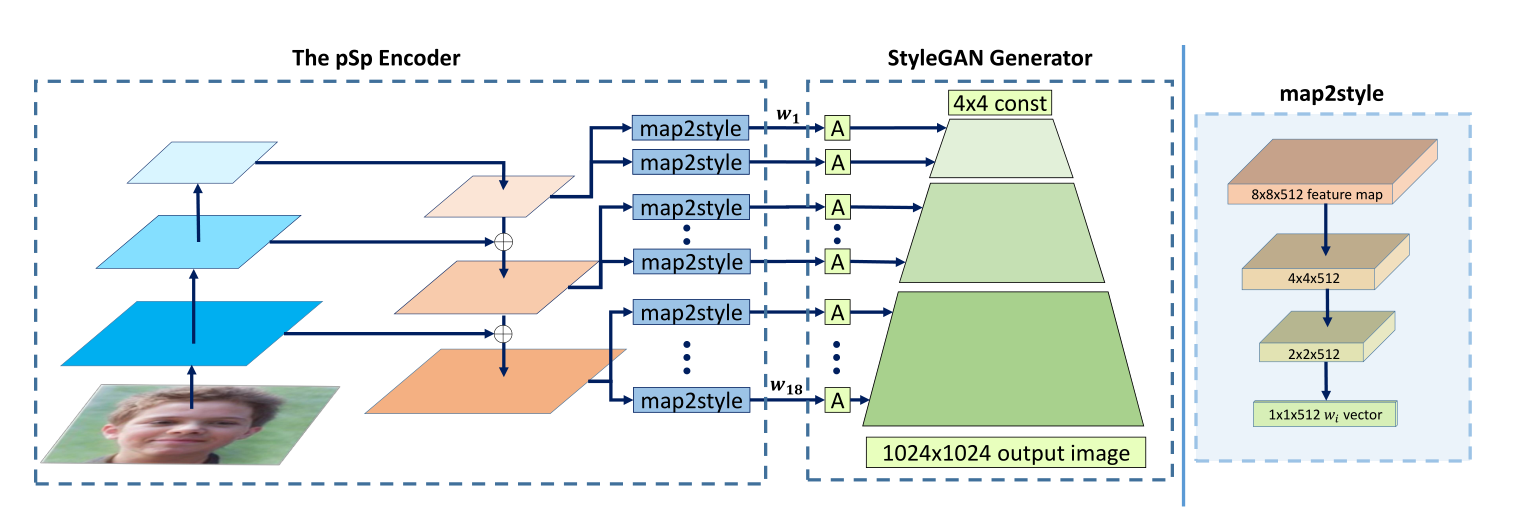
\includegraphics[width=0.8\textwidth]{img/m3p1.png} 
\caption{pSp 框架}
\label{Test}
\end{figure}
 
在整个架构中,只有Encoder部分是需要训练的,StyleGAN Generator部分使用的是预训练好的StyleGAN2的模型。首先,该编码器可以直接将真实图像嵌入到 W+ 中,无需额外优化。其次,编码器可以直接解决图像的转换任务。与之前StyleGAN编码器的“先反转,后编辑”的方法相比,pSp不要求输入图像在 StyleGAN 域中进行特征表示,可以直接将这些图像翻译任务编码成StyleGAN。该编码器极大地简化了训练过程,在没有图像对的标签下提供更好的支持,并且通过style的重采样可以支持多模态合成。与以往的工作通常依赖于专用的体系结构来解决单个翻译任务不同,pSp只需要对训练损失和方法进行微小的更改,就能够解决各种各样的问题。

\subsection{e4e 的 Designing an Encoder for StyleGAN Image Manipulation}

1. 背景和动机:

主要工作:提出什么样的encoder(image->latent code)具有更好的编辑性和更小的失真。
答案:图片逆映射接近W空间的encoder是好的。
要用利用预训练的stylegan进行图像编辑,需要将图像映射到stylegan的latent space。stylegan的latent space中存在两种权衡:
(1)扭曲-编辑权衡 distortion-editability tradeoff
(2)扭曲-感知权衡 distortion-perception tradeoff
stylegan的W空间具有丰富的解纠缠性质,可用于操作stylegan进行各种图像处理。然而,对任何图像用stylegan进行处理,必须首先将图像逆映射到W空间。高质量的反演(invert)方法对于编辑效果至关重要。
一个好的反演(图像->stylegan的W空间)具有的特性:
(1)inversion得到的latent code输入stylegan中能够恢复原图像
(2)能够最大程度地利用latent space的编辑能力
定义衡量重建性能的三个指标:
(1)editability
(2)distortion —— per-image input-output similarity
(3)perceptual quality —— how realistic the reconstructed image is
W 潜在空间的表达性已被证明是有限的,并不是每幅图像都能准确地映射到 W 中。为了克服这一局限性,Abdal等人证明了任何图像都可以逆映射成W的扩展部分,记为W+。W+中的每一个 style code 由许多 style vector 组成。

2. IDEA:

目前基于 styleGAN 的图像编辑,评判的标准有两个,重构出来的效果以及可编辑性的强弱,作者分别用 distortion(扭曲程度)和 editability(编辑能力)代表。很可惜的是,一般扭曲程度低的方法,编辑能力弱。这是因为找到的隐向量已经离stylegan的W空间很远了,不是一个分布。比如 image2style 就提出,在W+空间优化隐向量,可以重构出任意一行图像,不管是不是人脸图像,但可编辑能力大大降低。

作者认为,找到的隐向量为好的标准就是解决W空间。接近有两层含义:(1). 每个 style code 之间的方差小;(2) 每个 style code 都在 W 空间中。围绕以上两个原则,作者提出 e4e(encoder for editing),一个编码器,用于将指定图像映射到隐空间上,同时还提出了一个用于评判隐向量重构性能和可编辑性能的综合性指标。作者用 adversarial training和progressive training scheme 等技巧训练了一个 encoder,使得它能将图像逆映射后尽可能地“接近”W空间。本文的目的是设计编码器能够更好的对图像进行编辑。首先,由于图像失真,感知质量和图像的可编辑性存在紧密的联系。在一定程度上,图像失真与感知质量成负相关,图像失真和图像的可编辑性成负相关。此外,本文还发现如果图像的逆隐空间向量越接近原本的隐空间分布W,那么图像的感知质量和可编辑性便越好。

3. 贡献:

(1)分析了 StyleGAN 的复杂 latent space ,并对其结构提出了新的看法。

(2)展示了 (distortion) 扭曲(失真、歪曲、变形)、感知 (perception) 和可编辑性 (editability) 之间固有的权衡
。
(3)描述了这些权衡,并设计了两种编码器来控制它们。

(4)提出了 e4e,一个创新的编码器专门设计,允许对反转真实图像的接下来的编辑。

4. 主要方法:

图片逆映射接近 W 空间的 encoder 是好的。

一个好的encoder,需要输出空间接近W空间。想要做到这一点:

(1)可以优化每个风格向量的方差,让其尽量小,极限的情况是完全一样;

(2)并足够接近 stylegan 的 w 空间

 \begin{figure}[htb]
\centering 
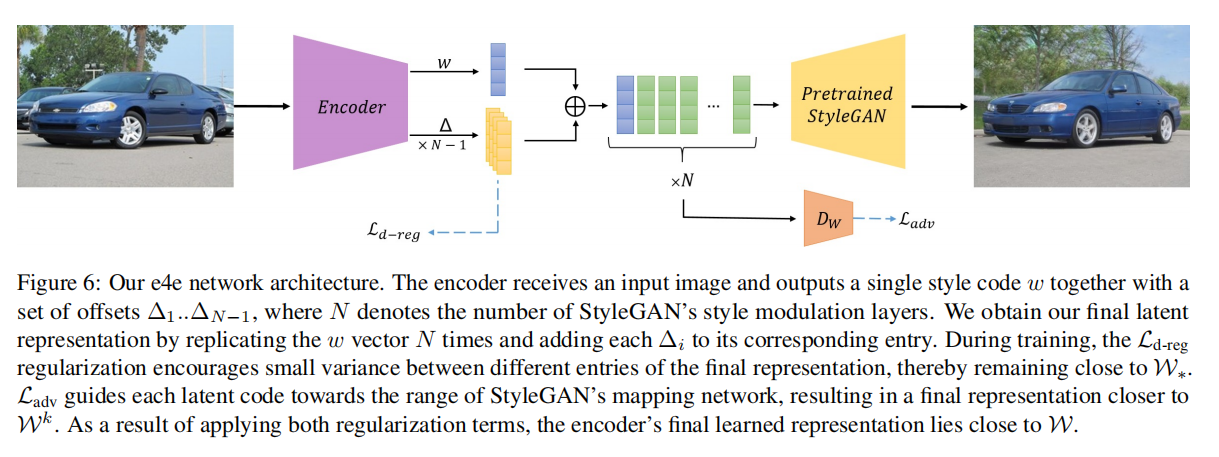
\includegraphics[width=0.8\textwidth]{img/m3p2.png} 
\caption{e4e 主要方法说明}
\label{Test}
\end{figure}

5. 优化方差

为了到达第一个目的,作者提出渐进训练方法。首先 encoder 记作E,输入是指定图像x。输出是 N 个style code。

\begin{equation}
E(x)=\left(w, \Delta_{1}, \ldots \Delta_{N-1}\right)
\end{equation}

后面N-1项是偏置,加在 w 上得到 N 个style code,具有不同的值,N 就是 stylegan 中的 style modulation 层的数目。该空间记作 $W^{k}_{\ast}$ 空间。在训练初期,让所有的偏置都为 0,这样 N 个向量都是相同的都是 w。即先鼓励 encoder 往 $W_{\ast}$ 空间上靠。然后逐渐的让偏置不一样,这样每个 style modulation 层都有不同的 style code,灵活性更高,保证了重构质量,实现了从 $W_{\ast}$  空间上 $W^{k}_{\ast}$ 的变化。其实如果偏置都为 0,encoder 也倾向于向 W 空间靠。但因为学习偏置的关系,离 W 空间也不远,也保证了可编辑的能力。距离由网络自己学习,自行权重可编辑性和重构性的 tradeoff。为了让偏置临近 $W_{\ast}$ 空间,作者设置了一个浅显易懂的正则损失:

\begin{equation}
\mathcal{L}_{\mathrm{d} \mathrm{dreg}}(w)=\sum_{i=1}^{N-1}\left\|\Delta_{i}\right\|_{2}
\end{equation}

6. 优化和 W 空间的距离

因为styleGAN的W空间并不能显式建模,所有作者使用了对抗思想,设置一个 latent code discriminator(Dw) 区分 encoder 的分布和W空间的分布。用同一个判别器,使用所有 N 个 style code 和真实的原始 W 空间向量。将 N 个 loss 求平均优化。

\begin{equation}
\begin{gathered}
\mathcal{L}_{\mathrm{adv}}^{D}=-\underset{w \sim \mathcal{W}}{\mathbb{E}}\left[\log D_{\mathcal{W}}(w)\right]-\underset{x \sim p_{X}}{\mathbb{E}}\left[\log \left(1-D_{\mathcal{W}}\left(E(x)_{i}\right)\right]+\right. \\
\underset{\frac{\gamma}{2}}{\mathbb{E}} \underset{w \sim \mathcal{W}}{\mathbb{E}}\left[\left\|\nabla_{w} D_{\mathcal{W}}(w)\right\|_{2}^{2}\right]
\end{gathered}
\end{equation}

\begin{equation}
\mathcal{L}_{\mathrm{adv}}^{E}=-\underset{x \sim p_{X}}{\mathbb{E}}\left[\log D_{\mathcal{W}}\left(E(x)_{i}\right)\right]
\end{equation}

\subsection{ReStyle: A Residual-Based StyleGAN Encoder via Iterative Refinement}

1. Topic:图像反演,获取潜在编码用于对图像进行直接编辑。

2. Problem:现在的单次编码架构无法准确的获得图像反推的潜在编码。即在重建精度方面,基于学习的反演方法与基于优化的反演方法仍存在较大差距。因此,虽然在基于学习的反演方面取得了显著的进展,但设计合适的编码器和训练方案仍然是一个挑战,许多工作仍在使用逐图像优化方法。

3. Idea:使用以残差为基础的迭代反馈调优架构。具体为将上一次迭代的输出与原始的输入图像共同输入到下一次迭代中,进行多次前向传播,让编码器注意到更多能够提升精度的特征。在增加有限的推理时间情况下,实现较高精度的输出。个人理解该方法是逐图像优化方法与编码器学习方法的折中。也是单步反演的松弛求解。

\begin{equation}
\hat{y}=G(E(x))
\end{equation}

其中 $x$ 为输入图像,$\hat{y}$ 为反演的图像, $G, E$ 分别为生成器和编码器。其具体工作如下:

4. Methods:

(1) 聚合真实图像和 Stylegan 的重建图像,生成六通道数据,然后输入到编码器中学习残差偏移编码。

(2) 更新图像 $x$ 的潜在编码,并输入到生成器中生成新重建图像。

(3) 其中初始的潜在编码和对应的潜在图像分别是训练好的生成器的平均风格向量和其对应生成图片。

 \begin{figure}[htb]
\centering 
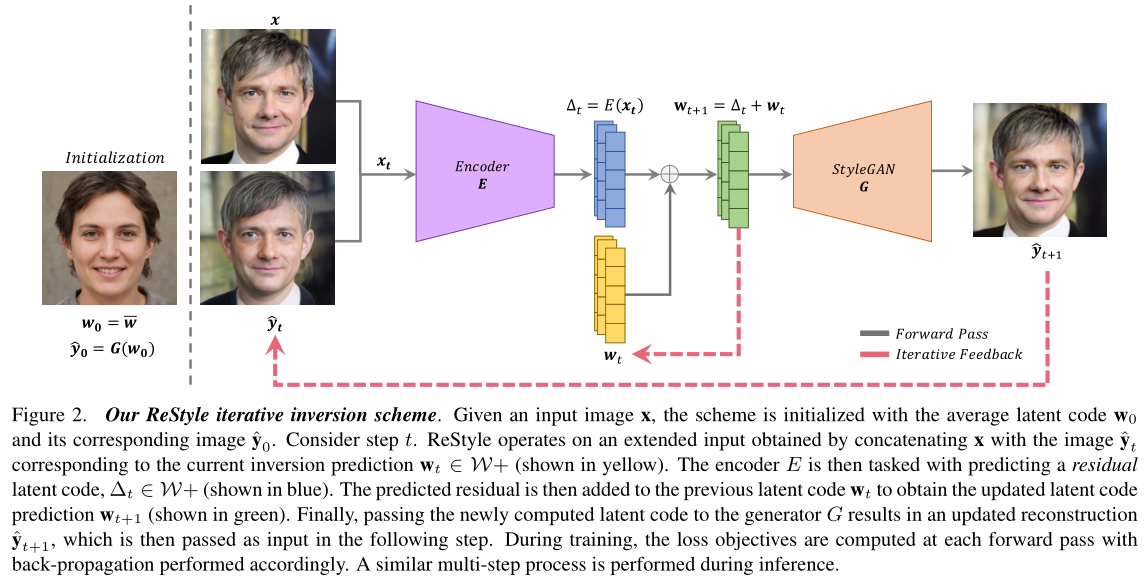
\includegraphics[width=0.8\textwidth]{img/m3p3.png} 
\caption{ReStyle 说明}
\label{Test}
\end{figure}

5. ReStyle 迭代反演方案

给定一个输入图像,用平均潜在码 $w_0$ 及其对应图像 ${\hat{y}}_0$ 作为初始化值。考虑t步的情况。ReStyle对一个扩展的输入进行操作,该输入通过将 $x$ 与对应于当前反转预测 $w_t\in W+$ 的图像 ${\hat{y}}_t$ (如图黄色部分所示)。然后,编码器E的任务是预测剩余潜在码,$∆t∈W+$(如图蓝色部分表示)。然后将预测残差加到前一个潜在码上,得到更新后的潜在码 $w_{t+1}$ (如图绿色所示)。最后,在更新的重构 ${\hat{y}}_{t+1}$ 中将新计算的潜在代码传递给生成器G生成的结果,然后在接下来的步骤中将其作为输入传递。在训练过程中,在每次前向传递时计算损失目标,并相应地进行反向传播。在推理过程中也会执行类似的多步骤过程。

6. 模型:

\begin{figure}[htb]
\centering 
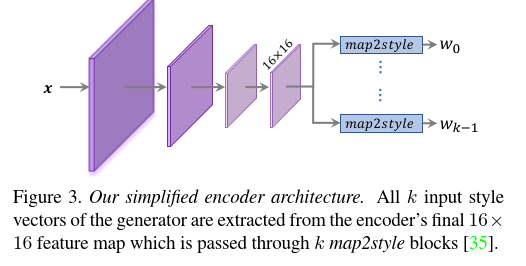
\includegraphics[width=0.8\textwidth]{img/m3p4.png} 
\caption{ReStyle 模型架构}
\label{Test}
\end{figure}

7. 编码器模型:因为迭代调优的特性, SOTA 工作中的特征金字塔和残差模块在该网络中并不需要。文中采用简单的特征下采样网络并结合 StyleGAN 的需要的风格输入作为输出,如 ReStyle 模型架构图。

\section{MetaFormer 及其相关原理介绍}

Transformer 与 2017 年由谷歌团队提出,其初衷是为了解决自然语言处理领域的问题。近年来,随着ViT模型首次将Transformer引入计算机视觉领域,其在视觉领域也开始显现出越来越大的潜力。早期人们普遍存在这样一种观点:Transformer 结构之所以能够取得这么大的成功,主要归功为注意力机制。因此,很多研究者对于注意力模块做了很多改进。然而,后续的研究发现即使在 Transformer 结构中不使用注意力机制,也同样可以取得很好的效果,例如 Spatial MLP 等等。在这种背景下,Meta-Former 得以提出。

\subsection{MetaFormer}

MetaFormer 的含义是对 Transformer 整体结构的一种抽象,因为作者认为:Transformer 中具体模块并不重要,重要的是它的整体架构。基于这种观点,作者将Attention机制抽象为一个信息混合和交换的模块。MetaFormer的具体结构如图中所示:左图是 Meta Former的整体结构,它不特指某一种具体的模型。右图是MetaFormer的具体结构模型,不同的是,Transformer采用了基于Attention的Token Mixer,而MLP-like模型采用的是Spatial MLP作为Token Mixer。为了验证作者的观点,作者还提出了一种结构极其简单的Pool Former,仅仅使用Pooling来代替Transformer中的注意力机制。

\begin{figure}[htb]
\centering 
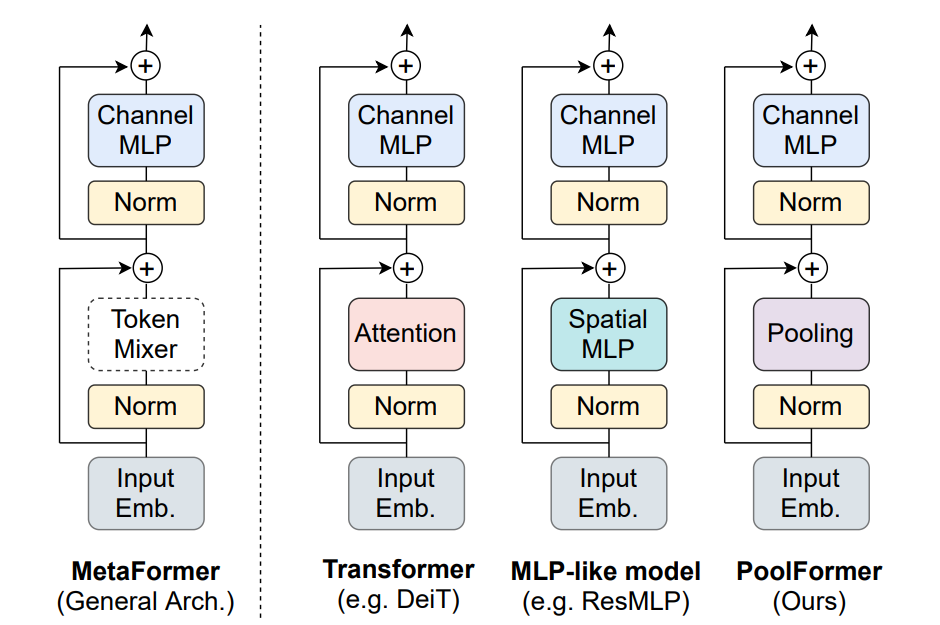
\includegraphics[width=0.8\textwidth]{img/m3p5.png} 
\caption{MetaFormer 的结构}
\label{Test}
\end{figure}

\subsection{PoolFormer}

同ViT的思路类似,Pool Former 首先进行 Patch embedding,通过 Patch embedding将图片单位化。之后结合金字塔结构,将整个模型分为几个不同的阶段,每一个阶段的 Patch size 逐渐提高,从而使得模型的整体感受野逐渐增大。图中 b 描述 了 PoolFormer block 的具体结构,可以看出其余 Transformer 结构基本类似,只是将其中的注意力机制变成了池化操作。通过这种极其简单的设计,Pool Former 同样在很多任务中取得了较好的效果,但是相比之下,它的参数量和浮点计算都要小得多。

\begin{figure}[htb]
\centering 
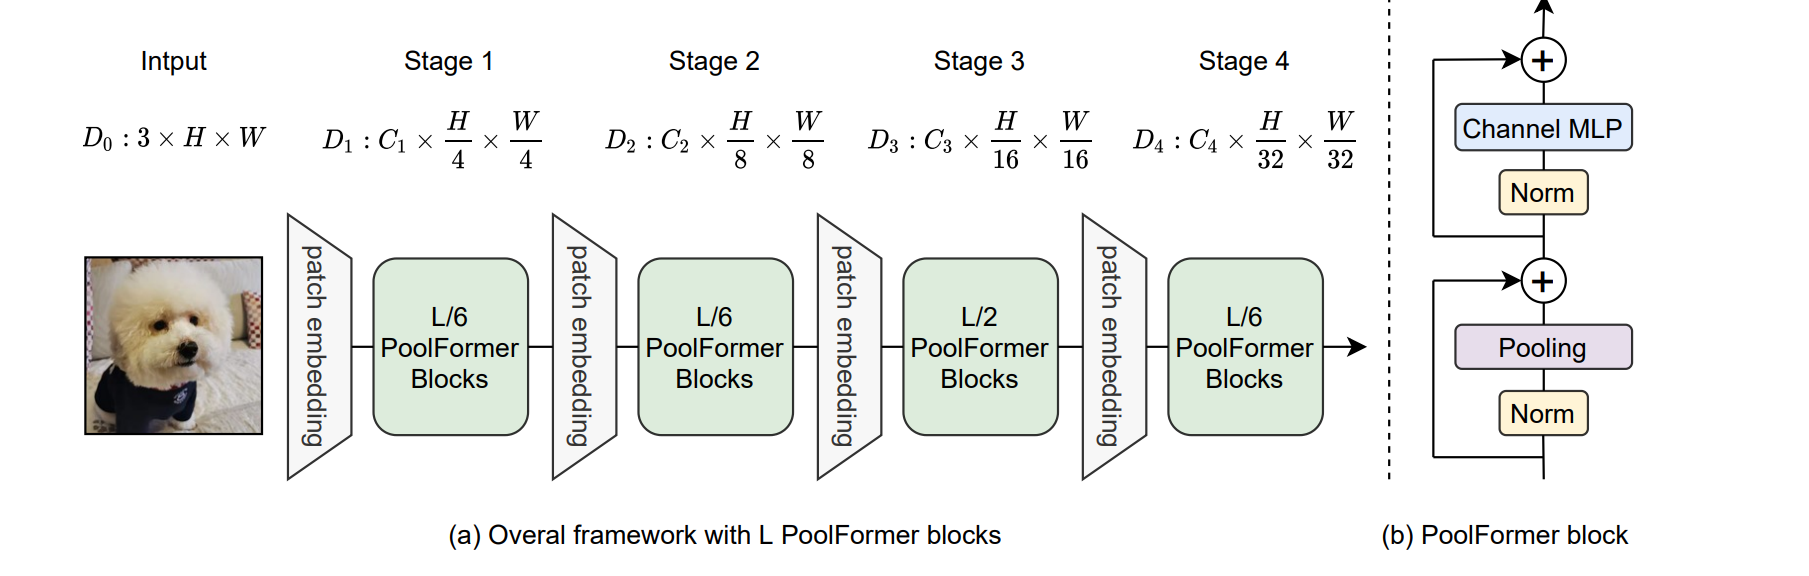
\includegraphics[width=0.8\textwidth]{img/m3p6.png} 
\caption{PoolFormer 的整体架构}
\label{Test}
\end{figure}

\subsection{PoolFormer 与 ReStyle-GAN 模型的结合}

基于 Transformer 在计算机视觉领域不断取得的重大突破,我们尝试将 Transformer 引入图像生成领域。PoolFormer结构简单,实现容易,并且容易在计算资源有限的条件下进行训练,因而我们选择将PoolFormer结构作为 ReStyle-GAN 网络的 Encoder,来尝试将类Transformer结构引入我们所研究的领域。下一步,我们将进行实验初步探索Pool Former 与 ReStyle-GAN 结合的效果,并在之后的探索中设计更加合理的 Former 结构,来对图像生成领域进行更深入的探索。

\section{实验条件、客观结果与分析}

\subsection{实验细节}
我们在所提出模型上进行了实验验证。所使用的显卡类型为 12G Titan Xp,所采用的深度学习框架为 Pytorch。实验采用高清人脸数据集(Flickr-Faces-High-Quality, FFHQ),其中含有 70000 张分辨率为 1024*1024 高清人脸数据,我们将训练集和测试集按照4:1划分:即 56000 张训练集,14000张测试集图片,并将其分辨率缩放为 256*256。训练阶段超参数如下:批次大小为 3,训练迭代轮次为 3,约 75000 次迭代。为保证实验一致性,我们设置 $\lambda_{/ 2}=1, \lambda_{\text {lpips }}=0.8$ 。
\subsection{对比模型}

为与所设计模型进行有效对比,我们选取了两个目前最佳的骨干网络模型进行了对比实验,分别为 ResNet34 和 ResNet152,其中 ResNet34 为原始 Restyle 模型的编码器。训练后的损失函数值如下表。通过下表,可见无论是逐像素的 $L_{2}$ 损失还是图片相似度损失 LPIPS,所设计架构在训练完成后的数值都比主流架构低,具体来说,所提出 PoolFormer 在 $L_{2}$ 损失和图片相似度损失 LPIPS 分别比 ResNet 低 6.62\% 和 4.96\% ,代表所设计模型具有良好的图片重构能力与风格转换能力,所生成图片像素信息和语义信息损失较少,主要原因为PoolFormer具有全局关注的注意力机制,较ResNet来说,PoolFormer 骨干网络能够更加全面地关注图片的风格特征。

\begin{table*}[htb]
    \centering
    \begin{minipage}[t]{0.55\linewidth} %
        \caption[模型损失函数值对比]{训练结束后模型损失函数值对比}
        \label{tab:example-table-basic}
        \begin{small}
        \begin{tabular}{@{}lccc@{}}
         \toprule[1.5pt]
        Encoder Architecture & $L_{2}$ Loss & LPIPS Loss \\
         \midrule[1pt]
          ResNet34 & 0.0302 & 0.2864 \\
          ResNet152 & 0.0269 & 0.2670 \\
          PoolFormer & 0.0282 & 0.2722 \\
          \bottomrule[1.5pt]
        \end{tabular}
        \end{small}
    \end{minipage}
\end{table*}

此外,我们还对比了模型之间的参数量和推断时间,用以反映所提出模型的效率,如表2。在相同软硬件平台上,PoolFormer在参数量更少的情况下,实现了更短时间的图片重建,其推断速度较Restyle提升了11.77\%,而参数量更少,进一步说明所设计模型相比 Restyle,图片重建效率更高。对比以 ResNet152 作为编码器的网络,PoolFormer 参数量远小于 ResNet152,而推断速度也约为其两倍。虽然训练后的重建损失略大,但是综合所提出模型的参数量和效率,PoolFormer 更优。

\begin{table*}[htb]
    \centering
    \begin{minipage}[t]{0.55\linewidth} %
        \caption[模型编码器参数量和图像重建时间]{模型编码器参数量和图像重建时间}
        \label{tab:example-table-basic}
        \begin{small}
        \begin{tabular}{@{}lccc@{}}
         \toprule[1.5pt]
        Encoder Architecture & 编码器参数量 (Mb) & 图像重建时间(秒) \\
         \midrule[1pt]
          ResNet34 & 216M & 0.17s \\
          ResNet152 & 581M & 0.31s \\
          PoolFormer & 209M & 0.15s \\
          \bottomrule[1.5pt]
        \end{tabular}
        \end{small}
    \end{minipage}
\end{table*}

\section{主观结果、主观分析}

\subsection{ReStyle 重建人脸图像}

此节图中所示为使用不同编码器的 ReStyle 重建人脸图像的结果。其中最左侧一列图像为原始图像,其余三列图像从左至右分别为第一至三次迭代重建的图像。从图中可以看出对于所有三种编码器,其对图像结构和语义的重建在第一次迭代就基本完成,后续的迭代主要是对图像的纹理细节进行提取和重建。三种编码器对图像语义特征的重建效果比较接近,但是可以看出基于 ResNet34 编码器提取特征的准确性明显低于其他两种编码器:其对面部表情特征的提取不够准确,同时也将图像左下角处的衣领误认为毛发。对于 ResNet152 编码器和 PoolFormer 编码器,可以看出 ResNet152 对毛发的纹理细节提取更为细节,这也是其 L2 和LPIPS误差较小的原因;PoolFormer 则对人脸中对一些皮肤细节进行了更好的提取,这在人脸的重建中是更为重要的。
但是使用三种编码器重建的人脸图像都出现了模糊的现象,这是使用L2损失训练编码器不可避免会出现的问题,我们认为原文在重建人脸图像时使用的身份损失和特征编码的正则化会有助于解决模糊现象。

\begin{figure}[htb]
\centering 
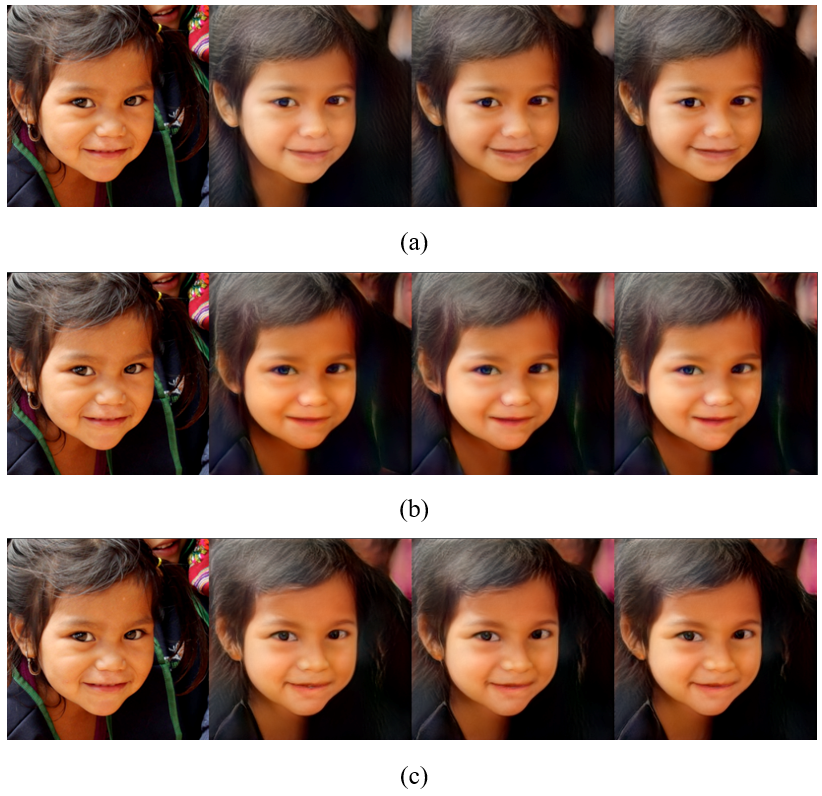
\includegraphics[width=0.8\textwidth]{img/m3p7.png} 
\caption{使用(a) ResNet34、(b) ResNet152、(c) PoolFormer作为编码器的ReStyle在FFHQ人脸数据集上的图像重建效果。最左侧一列为原始图像,其余三列从左至右分别为第一至三次迭代重建的图像。}
\label{Test}
\end{figure}

\subsection{不同编码器提取的人脸特征编码}

此节图中所示为使用不同编码器提取的人脸特征编码实现人脸混合的效果,使用最左侧一列原始图像中提取的底层人脸编码(决定结构特征)和最上方一行原始图像中提取的高层人脸编码(决定风格特征)生成图像。

可以看出,三种编码器中,PoolFormer 提取的特征更为准确,生成图像很好地保持了左侧图像的结构特征,并获取了上方图像的纹理特征,生成的图像在发色、肤色方面与上方图像基本一致。而使用ResNet编码器提取的特征出现了结构和风格耦合的现象,例如肤色和发色介于两张原始图像中间,或是混合了上方图像的一部分结构特征。

\begin{figure}[htb]
\centering 
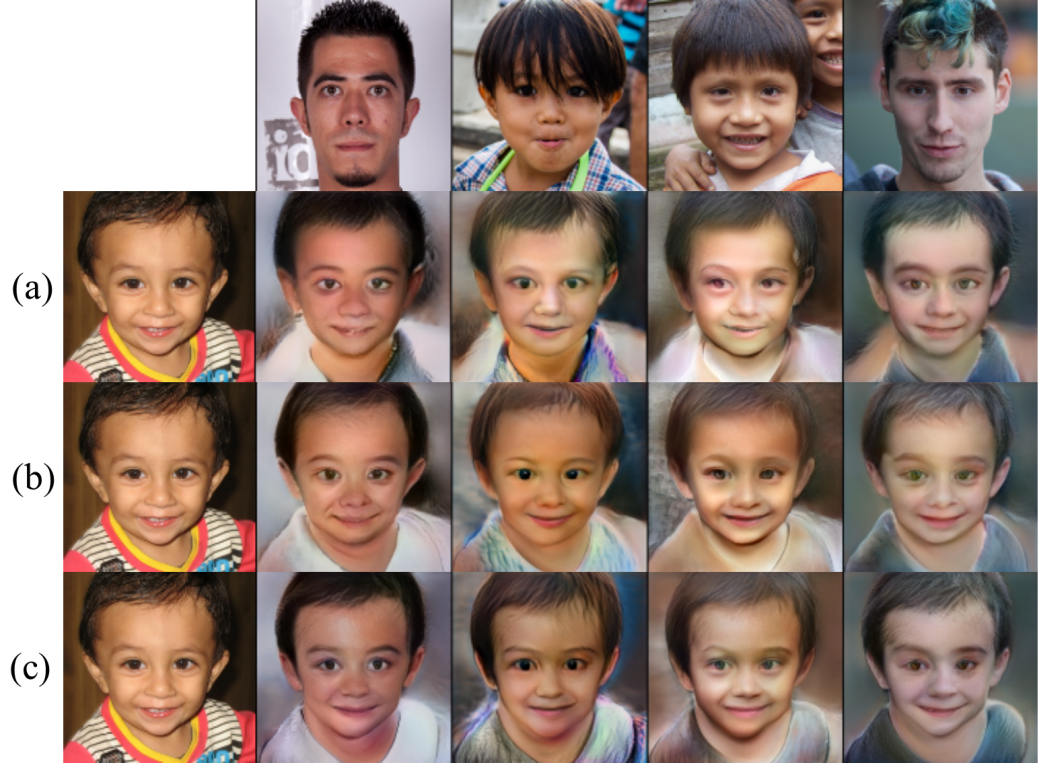
\includegraphics[width=0.8\textwidth]{img/m3p8.png} 
\caption{使用(a) ResNet34、(b) ResNet152、(c) PoolFormer作为编码器的ReStyle在FFHQ人脸数据集上的特征混合效果。}
\label{Test}
\end{figure}


% \section{缺点分析与启发}


